\section{Experiments}
\label{sec:experiments}

We use AgentJudgeBench to evaluate the extent to which LLM-judge alignment depends on the generator, query difficulty, and ground-truth availability. All protocol details (prompts, scoring, conditions) are in Section~\ref{sec:methodology}; model identifiers are in Appendix~\ref{app:generators} and Appendix~\ref{app:judges}.

\subsection{Experimental Setup}
\label{sec:exp:design}

We instantiate a fully-crossed factorial over three factors: generator $g \in \mathcal{G}$ (five models, 3B to frontier), judge $j \in \mathcal{J}$ (six LLMs), and difficulty $d \in \{\text{easy}, \text{medium}, \text{hard}\}$. Each cell is observed under both GT and no-GT conditions, yielding 90 factorial cells and $321{,}648$ valid (generator, judge, difficulty, record) tuples. Exact per-cell counts are in Appendix~\ref{app:eval-stats}. We report $\mathrm{align}(j, g, d, c)$ (Eq.~\ref{eq:alignment}) and, where relevant, GT lift (Eq.~\ref{eq:lift}).

\subsection{Results and Analysis}
\label{sec:exp:main}

Table~\ref{fig:full-results} reports every configuration in the factorial design. Each generator occupies a sub-block with six rows corresponding to the judges in $\mathcal{J}$. Columns pair each difficulty level with its GT and no-GT conditions. Bold entries mark the highest alignment within each (difficulty, condition) column of each sub-block.

\textbf{Finding 1: Monotone difficulty degradation.} All 30 (generator, judge) pairs exhibit strictly monotone alignment degradation from easy to hard under both GT and no-GT conditions (Table~\ref{fig:full-results}). No-GT degradation magnitude is roughly $1.5\times$ larger than GT degradation. On hard no-GT records, all six judges converge to a narrow $77$--$82\%$ band across four of five generators (including the frontier GPT-5.4 generator), indicating a task-level rather than judge-level ceiling. Difficulty degradation curves are in Appendix~\ref{app:degradation}.

\begin{figure*}[!htbp]
\centering

\resizebox{0.95\linewidth}{!}{%
  \setlength{\tabcolsep}{5pt}
  \renewcommand{\arraystretch}{1.05}
  \begin{tabular}{@{}ll cc cc cc@{}}
  \toprule
  & & \multicolumn{2}{c}{\textbf{Easy}}
    & \multicolumn{2}{c}{\textbf{Medium}}
    & \multicolumn{2}{c}{\textbf{Hard}} \\
  \cmidrule(lr){3-4}\cmidrule(lr){5-6}\cmidrule(lr){7-8}
  \textbf{Generator} & \textbf{Judge}
    & \textbf{GT} & \textbf{no-GT}
    & \textbf{GT} & \textbf{no-GT}
    & \textbf{GT} & \textbf{no-GT} \\
  \midrule

  \multirow{6}{*}{\textit{Llama-3.3-70B}}
    & GPT-5.4        & 91.4 & 95.2 & 87.4 & 91.7 & 83.0 & \textbf{84.6} \\
    & Claude         & 93.3 & 94.6 & 89.9 & 90.7 & 83.7 & 83.3 \\
    & Gemini-2.5-Pro & 90.5 & \textbf{95.7} & 86.5 & \textbf{92.2} & 82.2 & \textbf{84.6} \\
    & QwQ-32B        & \textbf{96.6} & 95.6 & \textbf{93.6} & 92.1 & \textbf{87.5} & 84.4 \\
    & GPT-OSS-20B    & 89.0 & 94.5 & 87.2 & 91.2 & 83.9 & 84.0 \\
    & GPT-OSS-120B   & 96.0 & 95.5 & 93.0 & 92.1 & 87.2 & 84.5 \\
  \midrule

  \multirow{6}{*}{\textit{Llama-3.1-8B}}
    & GPT-5.4        & 88.5 & 91.4 & 85.0 & 87.5 & 80.6 & \textbf{79.0} \\
    & Claude         & 90.3 & 90.6 & 86.5 & 86.6 & 80.3 & 77.1 \\
    & Gemini-2.5-Pro & 85.9 & \textbf{91.9} & 83.3 & \textbf{87.6} & 78.7 & 78.2 \\
    & QwQ-32B        & \textbf{94.2} & 91.2 & \textbf{90.8} & 86.8 & \textbf{84.1} & 76.6 \\
    & GPT-OSS-20B    & 87.4 & 89.5 & 85.3 & 85.7 & 81.2 & 75.9 \\
    & GPT-OSS-120B   & 93.1 & 90.7 & 89.8 & 86.6 & 83.6 & 76.6 \\
  \midrule

  \multirow{6}{*}{\textit{Qwen3-32B}}
    & GPT-5.4        & 90.5 & 93.9 & 86.4 & \textbf{89.4} & 81.9 & \textbf{81.7} \\
    & Claude         & 92.7 & 94.0 & 88.5 & 89.2 & 82.1 & 81.6 \\
    & Gemini-2.5-Pro & 86.4 & \textbf{94.1} & 83.0 & 89.2 & 78.1 & 81.4 \\
    & QwQ-32B        & \textbf{95.0} & 93.9 & \textbf{90.9} & 89.1 & \textbf{84.7} & 81.1 \\
    & GPT-OSS-20B    & 88.4 & 93.2 & 85.8 & 88.7 & 82.7 & 81.1 \\
    & GPT-OSS-120B   & 93.9 & 94.0 & 90.0 & 89.2 & 84.4 & 81.3 \\
  \midrule

  \multirow{6}{*}{\textit{SmolLM3-3B}}
    & GPT-5.4        & 86.0 & \textbf{87.3} & 81.6 & \textbf{82.0} & 76.9 & \textbf{73.3} \\
    & Claude         & 86.5 & 86.8 & 81.3 & 80.9 & 74.2 & 71.2 \\
    & Gemini-2.5-Pro & 81.1 & 86.6 & 77.7 & 80.7 & 73.4 & 70.8 \\
    & QwQ-32B        & \textbf{90.0} & 86.7 & \textbf{84.8} & 80.3 & 77.2 & 69.7 \\
    & GPT-OSS-20B    & 84.8 & 85.3 & 81.7 & 79.3 & 77.4 & 69.0 \\
    & GPT-OSS-120B   & 89.2 & 86.3 & \textbf{84.8} & 80.2 & \textbf{77.8} & 69.7 \\
  \midrule

  \multirow{6}{*}{\textit{GPT-5.4}}
    & GPT-5.4        & 85.8 & 87.0 & 84.1 & 84.9 & \textbf{81.4} & 79.8 \\
    & Claude         & \textbf{86.1} & \textbf{87.3} & \textbf{84.5} & \textbf{85.4} & 80.7 & \textbf{81.2} \\
    & Gemini-2.5-Pro & 81.6 & 85.2 & 80.2 & 83.3 & 77.6 & 78.4 \\
    & QwQ-32B        & 85.7 & 85.8 & 84.3 & 84.2 & 80.5 & 79.8 \\
    & GPT-OSS-20B    & 83.1 & 85.6 & 82.1 & 83.9 & 79.4 & 79.5 \\
    & GPT-OSS-120B   & 84.8 & 85.3 & 83.9 & 83.3 & 80.7 & 78.6 \\
  \bottomrule
  \end{tabular}%
  }
\caption{LLM–judge alignment (\%) with the programmatic reference, per (generator, judge, difficulty, condition). \textbf{GT}/\textbf{no-GT}: whether ground-truth tool calls are provided to the judge. Bold = column-wise maximum within each generator block. Bootstrap 95\% CIs (${\leq}0.7$\,pp half-width) in Appendix~\ref{app:bootstrap-ci}. DAG topology breakdown in Appendix~\ref{app:pertopology-table}; difficulty degradation curves and generator programmatic accuracy in Appendix~\ref{app:degradation}.}
\label{fig:full-results}

\end{figure*}

\textbf{Scope of Finding 1.} The medium$\to$hard drop (${\approx}5$--$7$\,pp GT) is the primary evidence for difficulty-driven degradation; hard rewrites are unanimously validated on $93.9\%$ of records (Appendix~\ref{app:rewrite-validation}), while the easy$\to$medium step (unanimous on $58.1\%$) partially reflects paraphrase-robustness. \\
\textbf{Finding 2: Ground-truth exposure is not monotonically beneficial.} GT lift (Eq.~\ref{eq:lift}) is positive for QwQ-32B and GPT-OSS-120B and reliably negative for GPT-5.4 and Gemini-2.5-Pro (non-overlapping bootstrap CIs; Appendix~\ref{app:bootstrap-ci}). Figure~\ref{fig:permetric} shows the effect concentrates in sequence accuracy: frontier judges anchor to the GT trace's ordering and penalise functionally equivalent but structurally deviant sequences. Case studies in Appendix~\ref{app:anchoring-cases}.

\textbf{C3 control.} Replacing the reference with a wrong GT from a different record confirms pure anchoring (Table~\ref{tab:c3-anchoring}): Gemini-2.5-Pro aligns identically under standard and corrupted GT; QwQ-32B tracks no-GT within $0.2$\,pp. Full results in Appendix~\ref{app:c3-table}.

\begin{wraptable}{r}{0.70\linewidth}
\vspace{-10pt}
\centering
\small
\setlength{\tabcolsep}{4pt}
\renewcommand{\arraystretch}{1.05}

\caption{C3 corrupted-GT control on Llama-3.3-70B generator. Alignment (\%) under standard GT, no-GT, and corrupted-GT (wrong reference from a different record). Gemini-2.5-Pro with corrupted GT matches standard GT on medium/hard, confirming reference-content anchoring. QwQ-32B with corrupted GT matches no-GT, confirming reference robustness.}
\label{tab:c3-anchoring}

\begin{tabular}{@{}llrrrl@{}}
\toprule
\textbf{Judge} & \textbf{Diff} & \textbf{GT} & \textbf{no-GT} & \textbf{Corrupt-GT} & \textbf{cGT$-$noGT} \\
\midrule
\multirow{3}{*}{QwQ-32B}
  & Easy   & 96.6 & 95.6 & 95.5 & $-0.1$ \\
  & Medium & 92.3 & 92.0 & 92.0 & $\phantom{-}0.0$ \\
  & Hard   & 84.6 & 84.4 & 84.6 & $+0.2$ \\
\midrule
\multirow{3}{*}{Gemini-2.5-Pro}
  & Easy   & 90.7 & 95.7 & 92.5 & $-3.2$ \\
  & Medium & 86.4 & 92.1 & 86.4 & $-5.7$ \\
  & Hard   & 78.9 & 84.6 & 78.9 & $-5.7$ \\
\bottomrule
\end{tabular}

\vspace{-12pt}
\end{wraptable}


\begin{figure*}[t]
\centering
  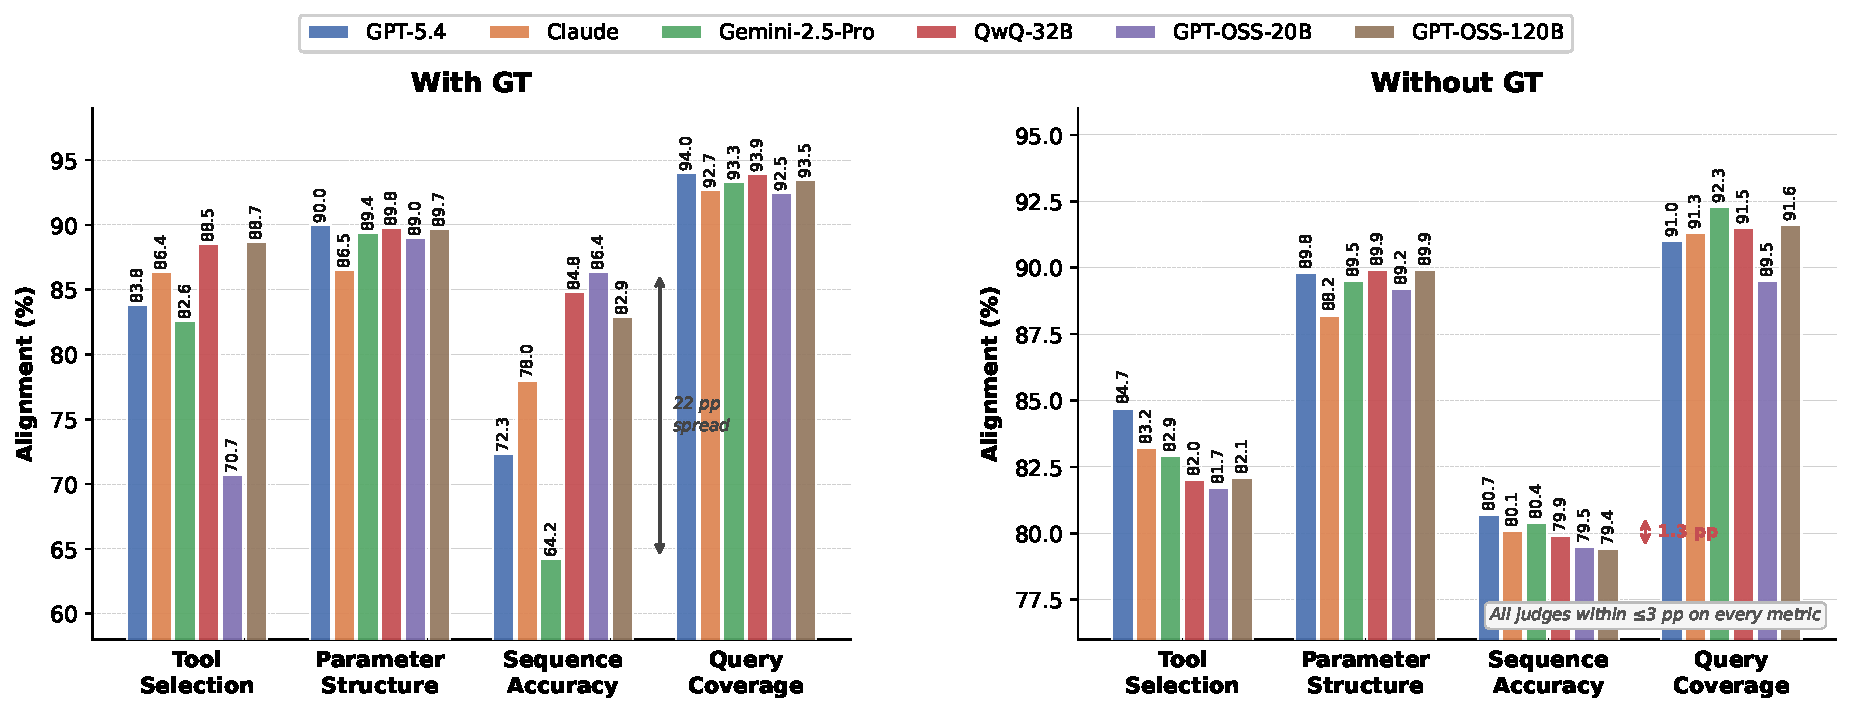
\includegraphics[width=\textwidth]{figures/per_metric_both.pdf}
  \caption{Per-metric alignment (with and without GT) across six judges. }
  \label{fig:permetric}
\end{figure*}

\textbf{Finding 3: Best judge depends on configuration.} QwQ-32B leads GT alignment in 10 of 15 (generator, difficulty) cells but is never the top no-GT judge; Gemini-2.5-Pro and GPT-5.4 lead no-GT on stronger and weaker generators respectively. See Appendix~\ref{app:decision-guide} for a deployment decision table.

The following RQs explain the mechanisms behind Findings 1--3.
\\
\textbf{RQ1: Which metrics and DAG topologies are hardest for judges?}
\label{sec:exp:disaggregation}

Figure~\ref{fig:permetric} breaks alignment into per-metric components. With GT, sequence accuracy is the weakest dimension with substantial inter-judge spread; without GT, all judges compress to a narrow per-metric band, reflecting the $1.0$-default rubric. DAG topology imposes a judge-independent difficulty ordering (\emph{fan\_out} easiest, \emph{loop\_like}/\emph{fan\_in} hardest); full numerical breakdowns in Appendix~\ref{app:permetric-table} and Appendix~\ref{app:pertopology-table}.

\textbf{RQ2: How much do judges agree with each other?}
\label{sec:exp:interjudge}

\begin{wraptable}{r}{0.72\textwidth}
\centering
\small
\vspace{-12pt}
\setlength{\tabcolsep}{4.5pt}
\renewcommand{\arraystretch}{1.05}
\caption{Pairwise inter-judge agreement under the with-GT condition.
\emph{Upper triangle}: exact metric-level agreement rate (\%).
\emph{Lower triangle}: Cohen's $\kappa$. Values computed over per-metric
verdicts aggregated across all 12 $(g, d)$ configurations.}
\label{tab:interjudge}
\begin{tabular}{@{}lcccccc@{}}
\toprule
 & \textbf{GPT-5.4} & \textbf{Claude} & \textbf{Gemini} & \textbf{QwQ-32B} & \textbf{OSS-20B} & \textbf{OSS-120B} \\
\midrule
GPT-5.4      & -   & 78.4  & 76.4  & 79.7  & 75.2  & 79.8  \\
Claude       & 0.430 & -   & 76.5  & 85.1  & 70.4  & 83.2  \\
Gemini       & 0.432 & 0.328 & -   & 80.7  & 74.5  & 81.6  \\
QwQ-32B      & 0.446 & 0.490 & 0.411 & -   & 77.4  & \textbf{89.4} \\
OSS-20B      & 0.419 & 0.225 & 0.387 & 0.386 & -   & 78.4  \\
OSS-120B     & 0.449 & 0.424 & 0.437 & \textbf{0.606} & 0.414 & -   \\
\bottomrule
\end{tabular}
\vspace{-12pt}
\end{wraptable}

Table~\ref{tab:interjudge} reports pairwise judge agreement. Mean agreement is $79.1\%$ ($\kappa=0.419$) with-GT and $92.6\%$ ($\kappa=0.559$) no-GT; the higher no-GT value reflects prompt-driven verdict compression rather than genuine consensus. The highest agreement is QwQ-32B$\times$GPT-OSS-120B ($89.4\%$, $\kappa=0.606$); the lowest is Claude$\times$GPT-OSS-20B ($70.4\%$, $\kappa=0.225$). Under no-GT, pairwise $\kappa$ decreases monotonically with judge tier separation ($\rho=-0.825$, $p<0.01$); this relationship vanishes under GT ($\rho=-0.171$), where ground truth acts as a shared anchor. Disagreement concentrates at the $0.5$ partial-credit boundary ($94$--$97\%$ of off-diagonal entries); verdict-level confusion matrices in Appendix~\ref{app:confusion}, binary scale ablation in Appendix~\ref{app:abl-binary}.

A soft jury of all six judges matches but does not exceed the top individual judge ($82.5\%$ with-GT hard)~\cite{verga2024jury}; ensemble and individual rankings against human annotators are in Appendix~\ref{app:prog-judge-validation}.

\textbf{RQ3: Why does no-GT alignment converge on hard queries?}
\label{sec:exp:ceiling}

The $77$--$82\%$ hard no-GT convergence (Table~\ref{fig:full-results}) has three consistent explanations: (1) the no-GT prompt defaults to $1.0$, suppressing hard-query discrimination; (2) generator error peaks on hard records, compressing all judges identically; (3) per-metric compression is uniform (Table~\ref{tab:e4-permetric}). The six-judge ensemble achieves $77.6\%$ — matching the best individual judge — confirming correlated failure driven by a shared structural property, not independent per-judge noise.

\begin{wraptable}{r}{0.48\linewidth}
\vspace{-8pt}
\centering
\small
\setlength{\tabcolsep}{5pt}
\renewcommand{\arraystretch}{1.05}

\caption{Hard no-GT alignment (\%) under the standard 1.0-default and the recalibrated 0.5-default prompts, averaged across six judges per generator. $\Delta$ = (0.5-default) $-$ (1.0-default).}
\label{tab:c2-ceiling}

\begin{tabular}{@{}lrrl@{}}
\toprule
\textbf{Generator} & \textbf{1.0-default} & \textbf{0.5-default} & \textbf{$\Delta$} \\
\midrule
Llama-3.3-70B & 84.3 & 84.7 & $+0.4$ \\
Qwen3-32B     & 81.4 & 82.4 & $+1.0$ \\
GPT-5.4       & 79.5 & 80.0 & $+0.5$ \\
Llama-3.1-8B  & 77.2 & 81.3 & $+4.1$ \\
SmolLM3-3B    & 70.6 & 76.2 & $+5.6$ \\
\bottomrule
\end{tabular}

\vspace{-10pt}
\end{wraptable}

\textbf{C2 ablation: 0.5-default no-GT prompt.} Table~\ref{tab:c2-ceiling} compares hard no-GT alignment under the standard $1.0$-default and a recalibrated $0.5$-default prompt. For the three strongest generators the delta is ${\leq}{+1.0}$\,pp, confirming structural task difficulty as the primary ceiling driver. For weaker generators ($+4.1$--$+5.6$\,pp), the $1.0$-default over-credits incorrect outputs; practitioners evaluating low-quality generators should consider the $0.5$-default prompt.


\begin{figure*}[!htbp]
\centering
\begin{minipage}[t]{0.48\textwidth}
  \centering
  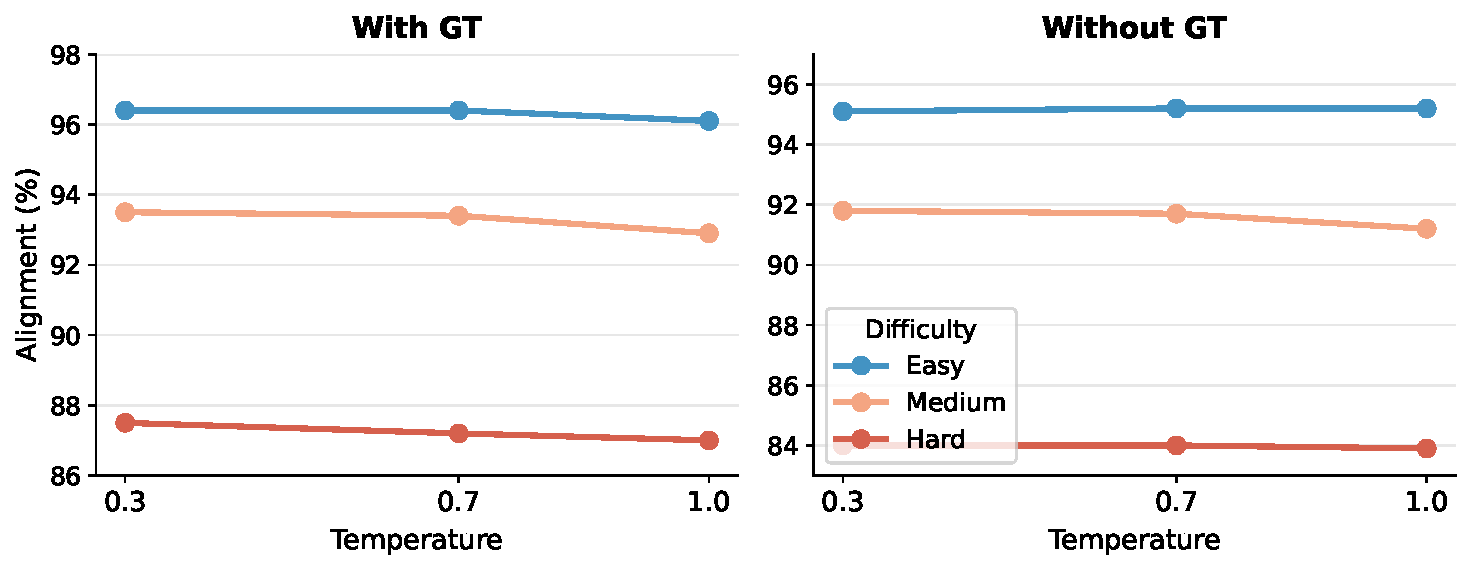
\includegraphics[width=\linewidth]{figures/abl_temperature.pdf}
  \captionof{figure}{%
    \textbf{Judge temperature sensitivity.}
    Qwen3-32B alignment at $T \in \{0.3, 0.7, 1.0\}$ on Llama-3.3-70B.
    All three difficulty curves are near-flat; maximum spread $\leq 0.6$\,pp.}
  \label{fig:abl-temperature}
\end{minipage}
\hfill
\begin{minipage}[t]{0.48\textwidth}
  \centering
  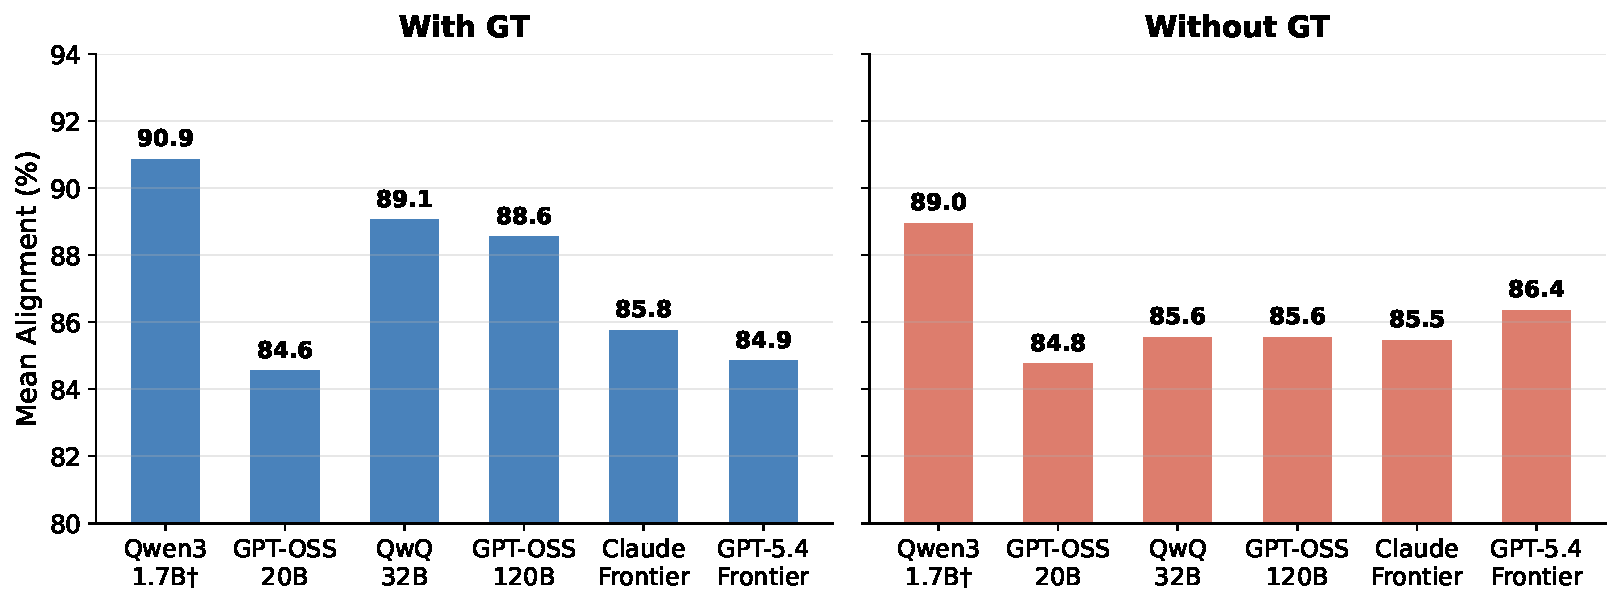
\includegraphics[width=\linewidth]{figures/abl_scale.pdf}
  \captionof{figure}{%
    \textbf{Judge scale vs.\ alignment.}
    Mean GT/no-GT alignment by model size (1.7B to frontier), averaged over the full 12-cell factorial per judge.
    No monotone scale law across families; within the GPT-OSS family, 120B exceeds 20B by 4\,pp.
    Qwen3-1.7B (84.3\%) is comparable to GPT-OSS-20B (84.6\%).}
  \label{fig:abl-scale}
\end{minipage}

\vspace{1em}

\begin{minipage}[t]{0.48\textwidth}
  \centering
  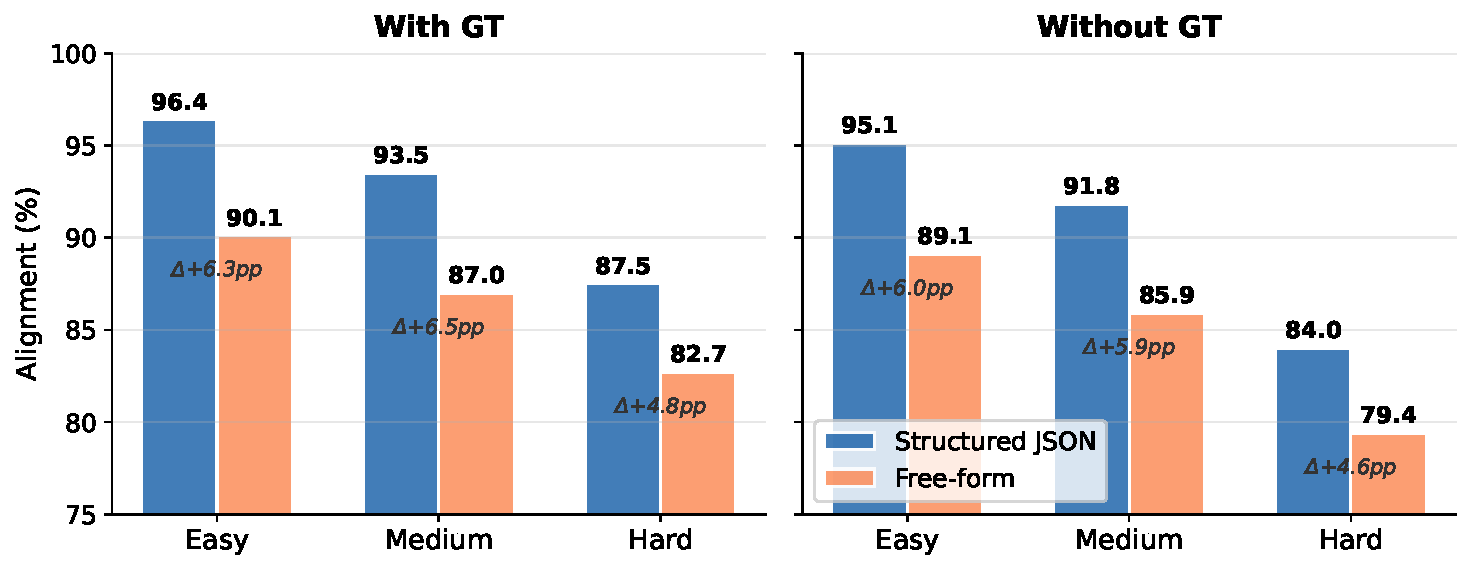
\includegraphics[width=\linewidth]{figures/abl_format.pdf}
  \captionof{figure}{%
    \textbf{Prompt structure vs.\ alignment.}
    Structured JSON prompt vs.\ free-form for Qwen3-32B on Llama-3.3-70B.
    The per-metric rubric adds $+4.8$-$+6.5$\,pp GT across all difficulty levels.}
  \label{fig:abl-format}
\end{minipage}
\hfill
\begin{minipage}[t]{0.48\textwidth}
  \centering
  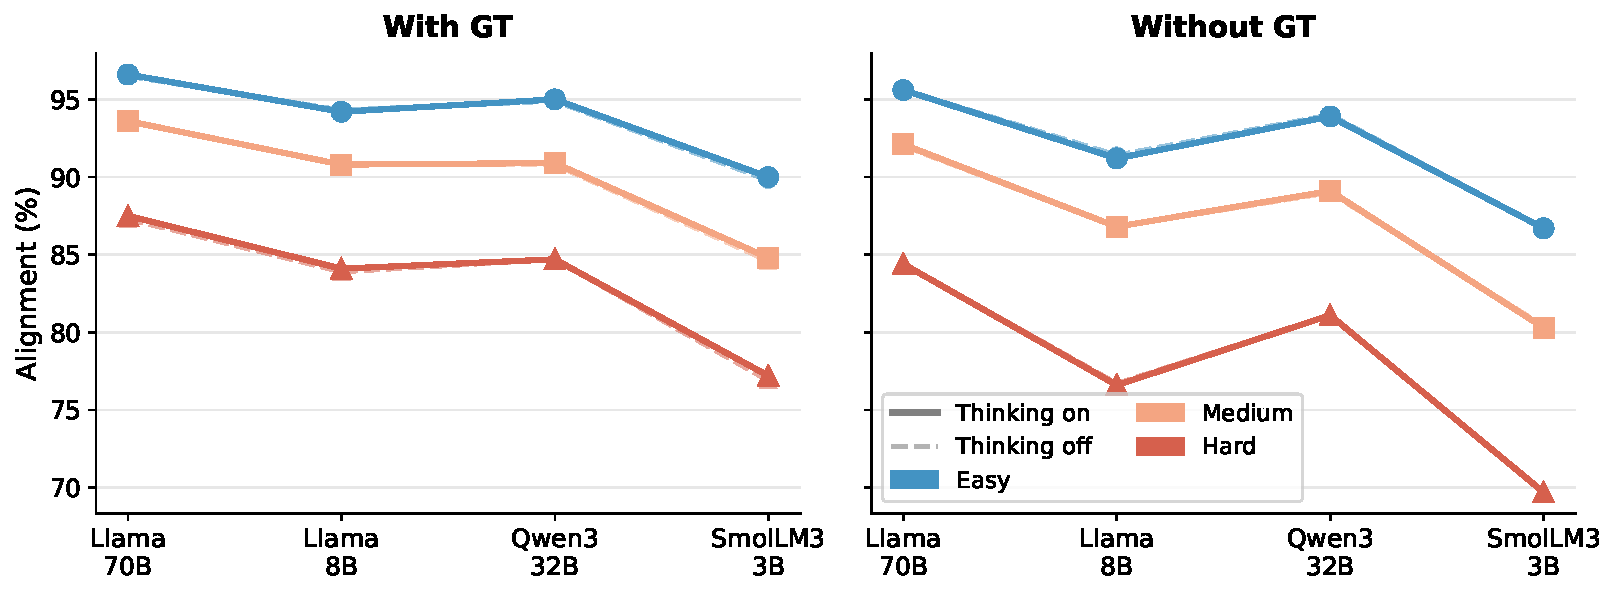
\includegraphics[width=\linewidth]{figures/abl_reasoning.pdf}
  \captionof{figure}{%
    \textbf{Chain-of-thought reasoning in the judge.}
    QwQ-32B with thinking on (solid) vs.\ off (dashed) across four open-weight generators.
    Curves are indistinguishable; maximum per-cell difference is $0.3$\,pp.}
  \label{fig:abl-reasoning}
\end{minipage}
\end{figure*}

\textbf{RQ4: Does judge temperature affect alignment?}
\label{sec:abl:temperature}

Figure~\ref{fig:abl-temperature} shows Qwen3-32B alignment is insensitive to temperature across $T \in \{0.3, 0.7, 1.0\}$: maximum spread $0.6$\,pp across all (difficulty, condition) cells. Structural pattern-matching dominates; full table in Appendix~\ref{app:ablations}.

\textbf{RQ5: Does judge model scale predict alignment?}
\label{sec:abl:scale}

Figure~\ref{fig:abl-scale} shows scale predicts alignment within families (GPT-OSS-120B exceeds GPT-OSS-20B by $4.0$\,pp GT) but not across families. Frontier judges underperform QwQ-32B on GT due to over-anchoring rather than capacity; full table in Appendix~\ref{app:ablations}.

\textbf{RQ6: Does prompt output format affect alignment?}
\label{sec:abl:format}

Figure~\ref{fig:abl-format} shows the structured per-metric JSON prompt outperforms a free-form variant by $+4.8$--$+6.5$\,pp GT across all difficulty levels, confirming prompt structure as a first-order alignment determinant. Full table in Appendix~\ref{app:ablations}.

\textbf{RQ7: Does chain-of-thought reasoning in the judge improve alignment?}
\label{sec:abl:reasoning}

Figure~\ref{fig:abl-reasoning} shows CoT reasoning contributes negligibly across 24 paired comparisons: mean GT gap $+0.11$\,pp, maximum per-cell $0.3$\,pp. QwQ-32B's advantage reflects training distribution rather than inference-time compute; full per-generator grid in Appendix~\ref{app:ablations}.
